W poprzednim rozdziale opisane zostały zagrożenia związane z publicznie znanymi podatnościami oraz sposób, w jaki radzą sobie organizacje w celu utrzymywania ryzyka na jak najniższym możliwym poziomie. Postawiona została teza pracy oraz zaproponowane modele ewaluacji.

\bigbreak
W niniejszym rozdziale przedstawiono wytworzone oprogramowanie Vulnerability Management Center (VMC), które powstało na potrzeby realizacji pracy doktorskiej w celu potwierdzenia tezy zawartej w rozdziale \ref{sec:zakres-i-teza-pracy}. Oprogramowanie VMC zostało opracowane z wykorzystaniem technologii, takich jak Docker \cite{anderson2015docker} i Kubernetes \cite{chemashkinkubernetes}, z wykorzystaniem algorytmu zaproponowanego w rozdziale \ref{sec:scaling}, dzięki czemu VMC jest dostosowane do rosnącej ilości napływających danych poprzez wykorzystanie mechanizmów skalowania. W dalszej części rozdziału przedstawiony został sposób implementacji parametrów $CDP$, $TD$, wykorzystana metoda konwersji oceny bazowej CVSS 2.0 do CVSS 3.x oraz metoda wykorzystana w analizie liczby oraz zakresu zmian w ocenach podatności.

\bigbreak
Przedstawione technologie oraz mechanizmy zaimplementowane w oprogramowaniu VMC przetestowane zostały w projekcie badawczym RegSoc \cite{regsoc}. Dodatkowo przed wdrożeniem oprogramowania wykonane zostały testy bezpieczeństwa i testy funkcjonalne przez firmę zewnętrzną, potwierdzające poprawność oraz stabilność przedstawionego rozwiązania. VMC od początku projektowane było jako system wspierający bezpieczeństwo monitorowanej infrastruktury teleinformatycznej w związku z czym, rozwijane było zgodnie z metodologią wytwarzania oprogramowania opartego na testach (ang. Test Driven Development, w skrócie TDD) \cite{astels2003test} z wykorzystaniem rekomendacji opisanych w Standardzie Weryfikacji Bezpieczeństwa Aplikacji OWASP (ang. Application Security Verification Standard, w skrócie ASVS) w wersji 4.0.2 poziom 2 \cite{ASVS}.

%%%%%%%%%%%%%%%%%%%%%%%%%%%%%%%%%%%%%%%%%%%%%%%%

%%%%%%%%%%%%%%%%%%%%%%%%%%%%%%%%%%%%%%%%%%%%%%%%
\section{Wprowadzenie do konteneryzacji}
\label{sec:docker}
Docker po raz pierwszy został zaprezentowany w 2013 roku na konferencji Python Developers \cite{bernstein2014containers}. W ciągu kilku tygodni od prezentacji pojawiło się duże zainteresowanie projektem, w związku z czym został on udostępniony na licencji otwartego oprogramowania (ang. open source) w serwisie Github. Docker to narzędzie, którego celem jest uproszczenie dystrybucji aplikacji, którą można wdrażać na dużą skalę w dowolnym środowisku. Docker ma na celu usprawnienie przepływu pracy oraz zwiększenie szybkości reagowania w organizacjach pracujących nad oprogramowaniem w modelu agile \cite{panthofer2019mastering}. Sama konteneryzacja nie jest niczym nowym, jednak przed wprowadzeniem Dockera \cite{anderson2015docker} była jedynie znana osobom, które profesjonalnie zajmowały się oprogramowaniem z wykorzystaniem niskopoziomowych koncepcji oferowanych przez Linux Kernel Containment (LXC). W chwili obecnej trudno jest znaleźć aplikację w której nie wspomina się lub nie wykorzystuje konteneryzacji. Docker przyspiesza cykle rozwoju oprogramowania, zmniejsza koszty infrastruktury, pomaga szybciej wdrażać nowych programistów, a nawet obniża bariery pomiędzy zespołami odpowiedzialnymi za rozwój oraz utrzymanie usług świadczonych przez organizacje. Docker nie zastępuje maszyny wirtualnej, natomiast jest jej dopełnieniem w architekturze chmurowej.

%%%%%%%%%%%%%%%%%%%%%%%%%%%%%%%%%%%%%%%%%%%%%%%%

%%%%%%%%%%%%%%%%%%%%%%%%%%%%%%%%%%%%%%%%%%%%%%%%
\subsection{Korzyści wynikające z zastosowania Dockera}
Niezwykle trudne jest wymienienie wszystkich zalet wykorzystania konteneryzacji. Samo skorzystanie z tej technologii przynosi już wiele korzyści dla samej organizacji, np. poprzez uproszczenie procesów wdrażania oprogramowania (Rysunek \ref{fig:chapter3:proces-without-docker}, \ref{fig:chapter3:proces-with-docker}). Docker ułatwia również podejmowanie decyzji dotyczącej architektury, ponieważ wszystkie aplikacje z punktu widzenia systemu operacyjnego, w którym są uruchomione, wyglądają dokładnie tak samo. Dodatkowo w literaturze można znaleźć korzyści, takie jak \cite{bernstein2014containers, chung2016using}:

\begin{itemize}
    \item \textbf{Tworzenie pakietów oprogramowania w sposób powtarzalny} - przed uproszczeniem sposobu konteneryzacji aplikacji wiele organizacji musiało utrzymywać dodatkowe stanowiska inżynierów odpowiedzialnych za tworzenie nowych wersji oraz kompilacji, aby zarządzać wiedzą i narzędziami niezbędnymi do przygotowywania pakietów oprogramowania dla wspieranych platform (np. osobno dla systemów Debian, Centos, itp). W przypadku Dockera, wszystkie wymagane pakiety w ramach jednego oprogramowania definiowane są w pojedynczym pliku odpowiedzialnym za budowanie obrazu docelowego (ang. Dockerfile), który bazuje na wybranej przez inżynierów oprogramowania, dystrybucji Linuksa.
    \item \textbf{Połączenie kodu aplikacji z niezbędnym systemem plików systemu operacyjnego w jednym obrazie o ustandaryzowanym formacie} - do poprawnego działania aplikacji trzeba dostarczyć również wiele niezbędnych bibliotek wymaganych do jej uruchomienia. Bez konteneryzacji niemożliwe było zapewnienie, że środowisko produkcyjne będzie działało w stu procentach identycznie jak środowisko programistyczne. W przypadku kompilowanego kodu oznaczało to, że systemy używane do budowania musiały mieć dokładnie takie same wersje bibliotek współdzielonych jak pozostałe środowiska. Wszystko to utrudniało tworzenie oprogramowania i było problemem dla wielu organizacji. Za pomocą Dockera dostarczana jest aplikacja zawierająca wszystkie niezbędne pliki oraz konfiguracje potrzebne do jej uruchomienia. Wykorzystując jedynie jądro systemu operacyjnego, na którym kontener jest uruchomiony, mamy pewność, że oprogramowanie będzie działało tak samo na wszystkich środowiskach.
    \item \textbf{Wykorzystanie pakietów do testowania i wdrażania dokładnie tego samego oprogramowania we wszystkich systemach i środowiskach} - Gdy programista wprowadza zmiany do systemu kontroli wersji, umożliwia utworzenie nowego obrazu Dockera, który przejdzie przez cały proces testowania i zostanie wdrożony w środowisku produkcyjnym bez potrzeby ponownego kompilowania go czy też przepakowywania na jakimkolwiek etapie, chyba że w danym przypadku jest to zachowanie pożądane \cite{virmani2015understanding}.
\end{itemize}

\begin{figure}[!ht]
\centering
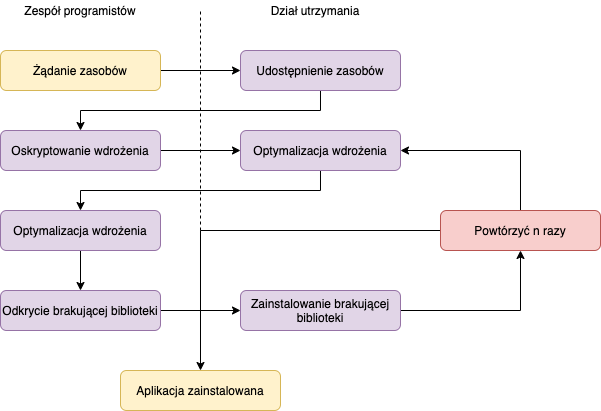
\includegraphics[width=.8\textwidth]{Chapters/Rozwiazanie/docker/proces-without-docker.png}
\caption{Przebieg tradycyjnego wdrożenia (bez Dockera).}
\label{fig:chapter3:proces-without-docker}
\end{figure}

\begin{figure}[!ht]
\centering
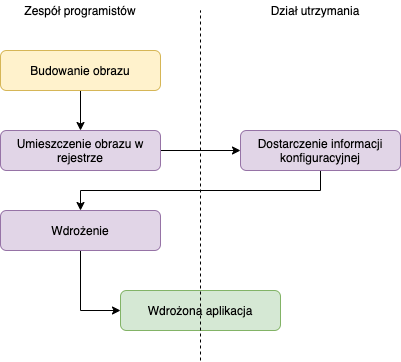
\includegraphics[width=.8\textwidth]{Chapters/Rozwiazanie/docker/proces-with-docker.png}
\caption{Przebieg wdrożenia z Dockerem.}
\label{fig:chapter3:proces-with-docker}
\end{figure}

%%%%%%%%%%%%%%%%%%%%%%%%%%%%%%%%%%%%%%%%%%%%%%%%

%%%%%%%%%%%%%%%%%%%%%%%%%%%%%%%%%%%%%%%%%%%%%%%%
\subsection{Czym Docker nie jest?}
Dzięki wykorzystaniu Dockera możliwe jest sprostanie wielu wyzwaniom, dla których tradycyjnie wykorzystywało się narzędzia innych kategorii. Szeroki zestaw możliwości często oznacza, że nie są dostępne bardzo specyficzne możliwości funkcjonalne. Na przykład w niektórych przypadkach pewne organizacje zauważą, że przy wykorzystaniu Dockera mogą zupełnie zrezygnować z narzędzi do zarządzania konfiguracją. Warto podkreślić, że Docker na pewno nie jest:

\begin{itemize}
    \item \textbf{Platformą do wirtualizacji (np. VMware, KVM)} - kontener nie jest maszyną wirtualną w tradycyjnym sensie. Maszyny wirtualne zawierają pełny system operacyjny działający pod kontrolą hiper nadzorcy zarządzanego przez system operacyjny serwera. Największą zaletą w porównaniu do sprzętowej wirtualizacji jest to, że w łatwy sposób można uruchomić wiele maszyn wirtualnych ze skrajnie różnymi systemami operacyjnymi na tym samym komputerze. Przy konteneryzacji zarówno główny system operacyjny, jaki i kontenery korzystają z tego samego jądra. To oznacza, że kontenery wykorzystują mniejszą ilość zasobów systemowych, ale muszą być oparte na tym samym systemie operacyjnym, zatem są mniej wymagające w stosunku do maszyn wirtualnych (Rysunek \ref{fig:chapter3:vm-vs-docker}).
    \item \textbf{Chmurą (np. Openstack, CloudStack)} - tak jak w przypadku wirtualizacji, wykorzystanie kontenerów wykazuje wiele podobieństw do korzystania z platform chmurowych. Oba te mechanizmy są tradycyjnie wykorzystywane, aby umożliwić horyzontalne skalowanie aplikacji w przypadku zmieniających się wymagań. Docker nie jest jednak platformą chmurową. Obsługuje jedynie wdrażanie, uruchamianie kontenerów i zarządzanie nimi na istniejących już komputerach z Dockerem. Nie pozwala na tworzenie nowych systemów (instancji), magazynów obiektów, urządzeń blokowych do przechowywania danych itp., jakie zazwyczaj zarządzane są przez platformę chmurową.
    \item \textbf{Zarządzaniem konfiguracją (np. Puppet, Chef) } - choć Docker znacząco usprawnia zarządzanie aplikacjami i ich zależnościami w organizacji, nie zastępuje bezpośrednio tradycyjnych systemów do zarządzania konfiguracją. W plikach Dockera definiuje się, jak kontener powinien wyglądać przy kompilacji, ale nie służą one do zarządzania późniejszym stanem kontenera i nie mogą być wykorzystywane do zarządzania systemem operacyjnym.
    \item \textbf{Frameworkiem do wdrażania (np. Capistrano, Fabric)} - Docker upraszcza wiele aspektów wdrażania aplikacji dzięki tworzeniu obrazów kontenerów, które zawierają wszystkie zależności aplikacji, w taki sposób, że mogą być one wdrożone w każdym środowisku bez modyfikacji. Docker nie może być jednak wykorzystany do automatyzacji złożonych procesów wdrażania. Potrzebne są nadal inne narzędzia pozwalające połączyć i zautomatyzować większe procesy.
    \item \textbf{Systemem do zarządzania obciążeniem (Mesos, Kubernetes, Swarm)} - dodatkowa warstwa koordynująca musi zostać wykorzystana do inteligentnego skoordynowania pracy większych grup serwerów z Dockerem, śledzenie stanu wszystkich serwerów oraz ich zasobów, a także rejestrowania działających kontenerów.
\end{itemize}

\begin{figure}[!ht]
\centering
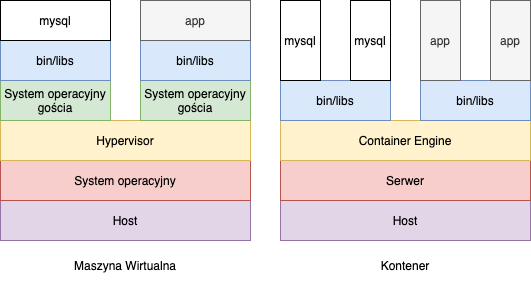
\includegraphics[width=.8\textwidth]{Chapters/Rozwiazanie/docker/vm-vs-docker.png}
\caption{Porównanie maszyny wirtualnej z kontenerem.}
\label{fig:chapter3:vm-vs-docker}
\end{figure}

\FloatBarrier

%%%%%%%%%%%%%%%%%%%%%%%%%%%%%%%%%%%%%%%%%%%%%%%%

%%%%%%%%%%%%%%%%%%%%%%%%%%%%%%%%%%%%%%%%%%%%%%%%
\section{Systemy do zarządzania kontenerami w środowisku chmurowym}
\label{sec:k8s}
Podczas wykorzystywania mechanizmu kontenerów w postaci silnika Docker inżynierowie zwrócili uwagę na problem koordynacji wielu pojedynczych serwerów z Dockerem i efektywnego wypełniania tych serwerów kontenerami. Powstało wiele narzędzi do zarządzania kontenerami w celu jak najefektywniejszego wykorzystania zasobów oferowanych przez klastry Dockerowe, takich jak Docker Swarm \cite{naik2016building}, Mesos \cite{mesos}, Centurion \cite{centurion} czy Kubernetes \cite{burns2018kubernetes}. W chwili obecnej na rynku komercyjnym liczą się tylko dwa rozwiązania: Docker Swarm oraz Kubernetes; ze znaczną przewagą tego drugiego, który obecnie dostarczany jest jako oprogramowanie usługa (ang. Software as a Service, w skrócie SaaS) przez wszystkich dostawców rozwiązań chmurowych \cite{chemashkinkubernetes}. 

\bigbreak
Kubernetes został zaprezentowany podczas konferencji DockerCon w 2014 roku przez firmę Google i od tego czasu dynamicznie się rozwija. Sama platforma dostępna jest dla wielu dystrybucji Linuxa. System do zarządzania kontenerami w środowisku chmurowym zapewnia między innymi:
\begin{itemize}
    \item \textbf{Detekcje nowych serwisów i balansowanie ruchu} - pozwala na udostępnienie kontenera, używając nazwy DNS lub swojego własnego adresu IP. Jeśli ruch przychodzący do kontenera jest zbyt duży, system może balansować obciążenie i przekierować ruch sieciowy, aby zapewnić stabilność całej instalacji (Rysunek \ref{fig:chapter3:lb}).
    \item \textbf{Zarządzenie obsługą składowania danych} - umożliwia automatyczne monitorowanie systemów składowania danych dowolnego typu.
    \item \textbf{Automatyczne wdrożenia i wycofywanie zmian} - można opisać oczekiwany stan instalacji, system sam zajmie się doprowadzeniem w sposób kontrolowany stanu faktycznego do stanu oczekiwanego. Przykładowo można zautomatyzować proces tworzenia nowych kontenerów na potrzeby wdrożenia oraz usuwania istniejących już kontenerów oraz zwalniania zasobów przez nie wykorzystywanych.
    \item \textbf{Automatyczne zarządzanie dostępnymi zasobami} - zadaniem administratora jest dostarczenie klastra maszyn, które można wykorzystać do uruchamiania zadań w kontenerach. Administrator określa zapotrzebowanie na moc procesora i pamięć RAM dla każdego z wykorzystywanych kontenerów. System sam rozmieszcza kontenery na maszynach w taki sposób, aby jak najlepiej wykorzystać dostarczone zasoby.
    \item \textbf{Samoczynne naprawianie} - system sam restartuje kontenery, które przestały działać, wymienia je na nowe i wymusza wyłączenie kontenerów, które nie działają, po czym poinformuje o dostępności nowych kontenerów, kiedy będą gotowe do działania. Dzięki czemu możliwe jest zbudowanie klastra, który będzie dostępny w dwóch osobnych lokalizacjach, tym samym lepiej wspierając wysoką dostępność (Rysunek \ref{fig:chapter3:ha}).
    \item \textbf{Zarządzanie informacjami poufnymi oraz konfiguracją} - system pozwala na składowanie oraz zarządzanie informacjami poufnymi, takimi jak hasła, tokeny API oraz klucze SSH. Informacje te mogą być dostarczane do aplikacji i zmieniane bez konieczności ponownego budowania obrazu kontenera i bez ujawniania poufnych danych w ogólnej konfiguracji oprogramowania.
\end{itemize}

\begin{figure}[!ht]
\centering
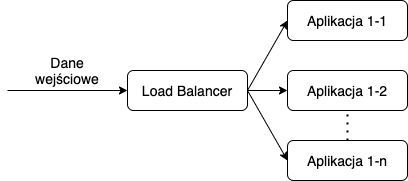
\includegraphics[width=.8\textwidth]{Chapters/Rozwiazanie/k8s/lb.png}
\caption{Wykorzystanie automatycznego mechanizmu równoważenia obciążenia (ang. Load Balancing).}
\label{fig:chapter3:lb}
\end{figure}

\begin{figure}[!ht]
\centering
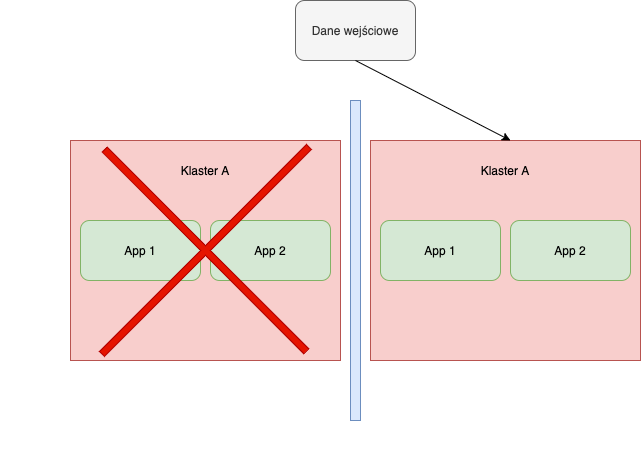
\includegraphics[width=.8\textwidth]{Chapters/Rozwiazanie/k8s/ha.png}
\caption{Mechanizm wysokiej dostępności.}
\label{fig:chapter3:ha}
\end{figure}

System zarządzania kontenerami dodatkowo:
\begin{itemize}
    \item Nie ogranicza typów aplikacji, które są obsługiwane. Celem systemu jest możliwość obsługi bardzo różnorodnego typu zadań, wliczając w to aplikacje bezstanowe (ang. stateless), aplikacje ze stanem (ang. stateful) i ogólne przetwarzanie danych.
    \item Nie oferuje wdrażania aplikacji wprost z kodu źródłowego i nie buduje aplikacji.
    \item Nie dostarcza warstwy aplikacyjnej, pośredniej (ang. middleware), np. broker wiadomości typu Rabbitmq, oraz funkcjonalności baz danych.
    \item Nie wymusza użycia konkretnych systemów zbierania logów, monitorowania ani ostrzegania.
    \item Nie dostarcza ani nie wymusza języka/systemu używanego do konfiguracji.
\end{itemize}

\bigbreak
Dzięki powyższym założeniom Kuberenetes pozwala na zbudowanie elastycznych i wysoko skalowalnych rozwiązań, dzięki czemu jest wykorzystywany również przez takie firmy jak Facebook, Twitter czy też Netflix \cite{vergilio2019non}.

%%%%%%%%%%%%%%%%%%%%%%%%%%%%%%%%%%%%%%%%%%%%%%%%

%%%%%%%%%%%%%%%%%%%%%%%%%%%%%%%%%%%%%%%%%%%%%%%%
\section{Opracowane oprogramowanie}
\label{sec:vmc}
Na potrzeby pracy autor stworzył oprogramowanie Centrum Zarządzania Podatnościami (ang. Vulnerability Management Center, w skrócie VMC), za pomocą którego przeprowadzono analizę zaproponowanych modeli zarządzania podatnościami \cite{vmcgithub}. W dalszej części pracy posługiwano się skrótem pochodzącym z języka angielskiego, gdyż jest on ogólnie przyjęty w opublikowanej przez autora literaturze. Oprogramowanie VMC wykorzystuje omówione wcześniej technologie w rozdziale \ref{sec:docker} oraz \ref{sec:k8s} i składa się z czterech głównych modułów: moduł pobierający informacje o podatnościach z publicznych baz danych (ang. Knowledge Collector), moduł pobierający informacje o zasobach infrastruktury teleinformatycznej (ang. Asset Collector), moduł pobierający informacje o wykrytych podatnościach w infrastrukturze teleinformatycznej (ang. Vulnerability Collector) oraz moduł obliczeniowy (ang. Processing Module). Rysunek \ref{fig:chapter3:vmc-arch} przedstawia architekturę VMC, które składają się na całość oprogramowania. Kolorem zielonym oznaczono komponenty, napisane przez autora pracy. Kolorem niebieskim komponenty, które są dostarczane przez firmy trzecie. Kolorem szarym dane wejściowe. Cały kod oprogramowania dostępny jest w publicznym repozytorium Github \cite{vmcgithub}. Dokładny opis instalacji oraz konfiguracji systemu dostępny jest w załącznikach dołączonych do niniejszej pracy.

\begin{figure}[!ht]
  \centering
  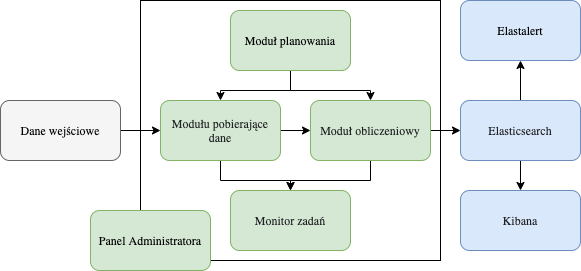
\includegraphics[width=.9\textwidth]{Chapters/Rozwiazanie/vmc/vmc-arch.png}
  \caption{Architektura VMC.}
  \label{fig:chapter3:vmc-arch}
\end{figure}

\bigbreak
Wszystkie moduły pracują niezależnie od siebie w myśl idei rozwiązań mikro serwisowych, komunikując się asynchronicznie za pomocą systemu kolejek \cite{johansson2020rabbitmq}. Dzięki czemu, w zależności od ilości danych przyjmowanych przez moduł, może być on skalowalny, niezależnie od pozostałych komponentów. 

\bigbreak
System konfigurowany jest z panelu administratora. Moduł planowania (ang. Scheduler) odpowiada za kolejność oraz czas pobierania danych z poszczególnych źródeł. Natomiast w monitorze zadań (ang. Task Monitor) można podejrzeć aktualny stan zadań wykonywanych w systemie. Dane przechowywane są w Elasticsearch \cite{gheorghe2015elasticsearch}, który umożliwia ich przetwarzanie w trybie pełnotekstowym, natomiast do warstwy prezentacji wyników wykorzystywane jest narzędzie Kibana \cite{gupta2015kibana}. Do implementacji niżej opisanych komponentów wykorzystany został język Python \cite{pilgrim2009dive} ze względu na jego elastyczność oraz możliwość wydajnego przetwarzania danych po stronie serwera. Cały projekt uwzględnia obsługę mulit-klientów (ang. tenants) oraz pozwala na pełną separację danych pomiędzy określonymi klientami. VMC działa w dwóch trybach: operacyjnym oraz historycznym. Tryb operacyjny pozwala użytkownikowi na podgląd wszystkich zaobserwowanych przez system zmian w czasie rzeczywistym, z kolei tryb historyczny umożliwia przeglądanie oraz wykonywanie operacji obliczeniowych na danych historycznych, poprawiając tym samym jakość i zakres analizy zdarzeń w systemie oraz w monitorowanej infrastrukturze teleinformatycznej.

\begin{figure}[thb]
\centering
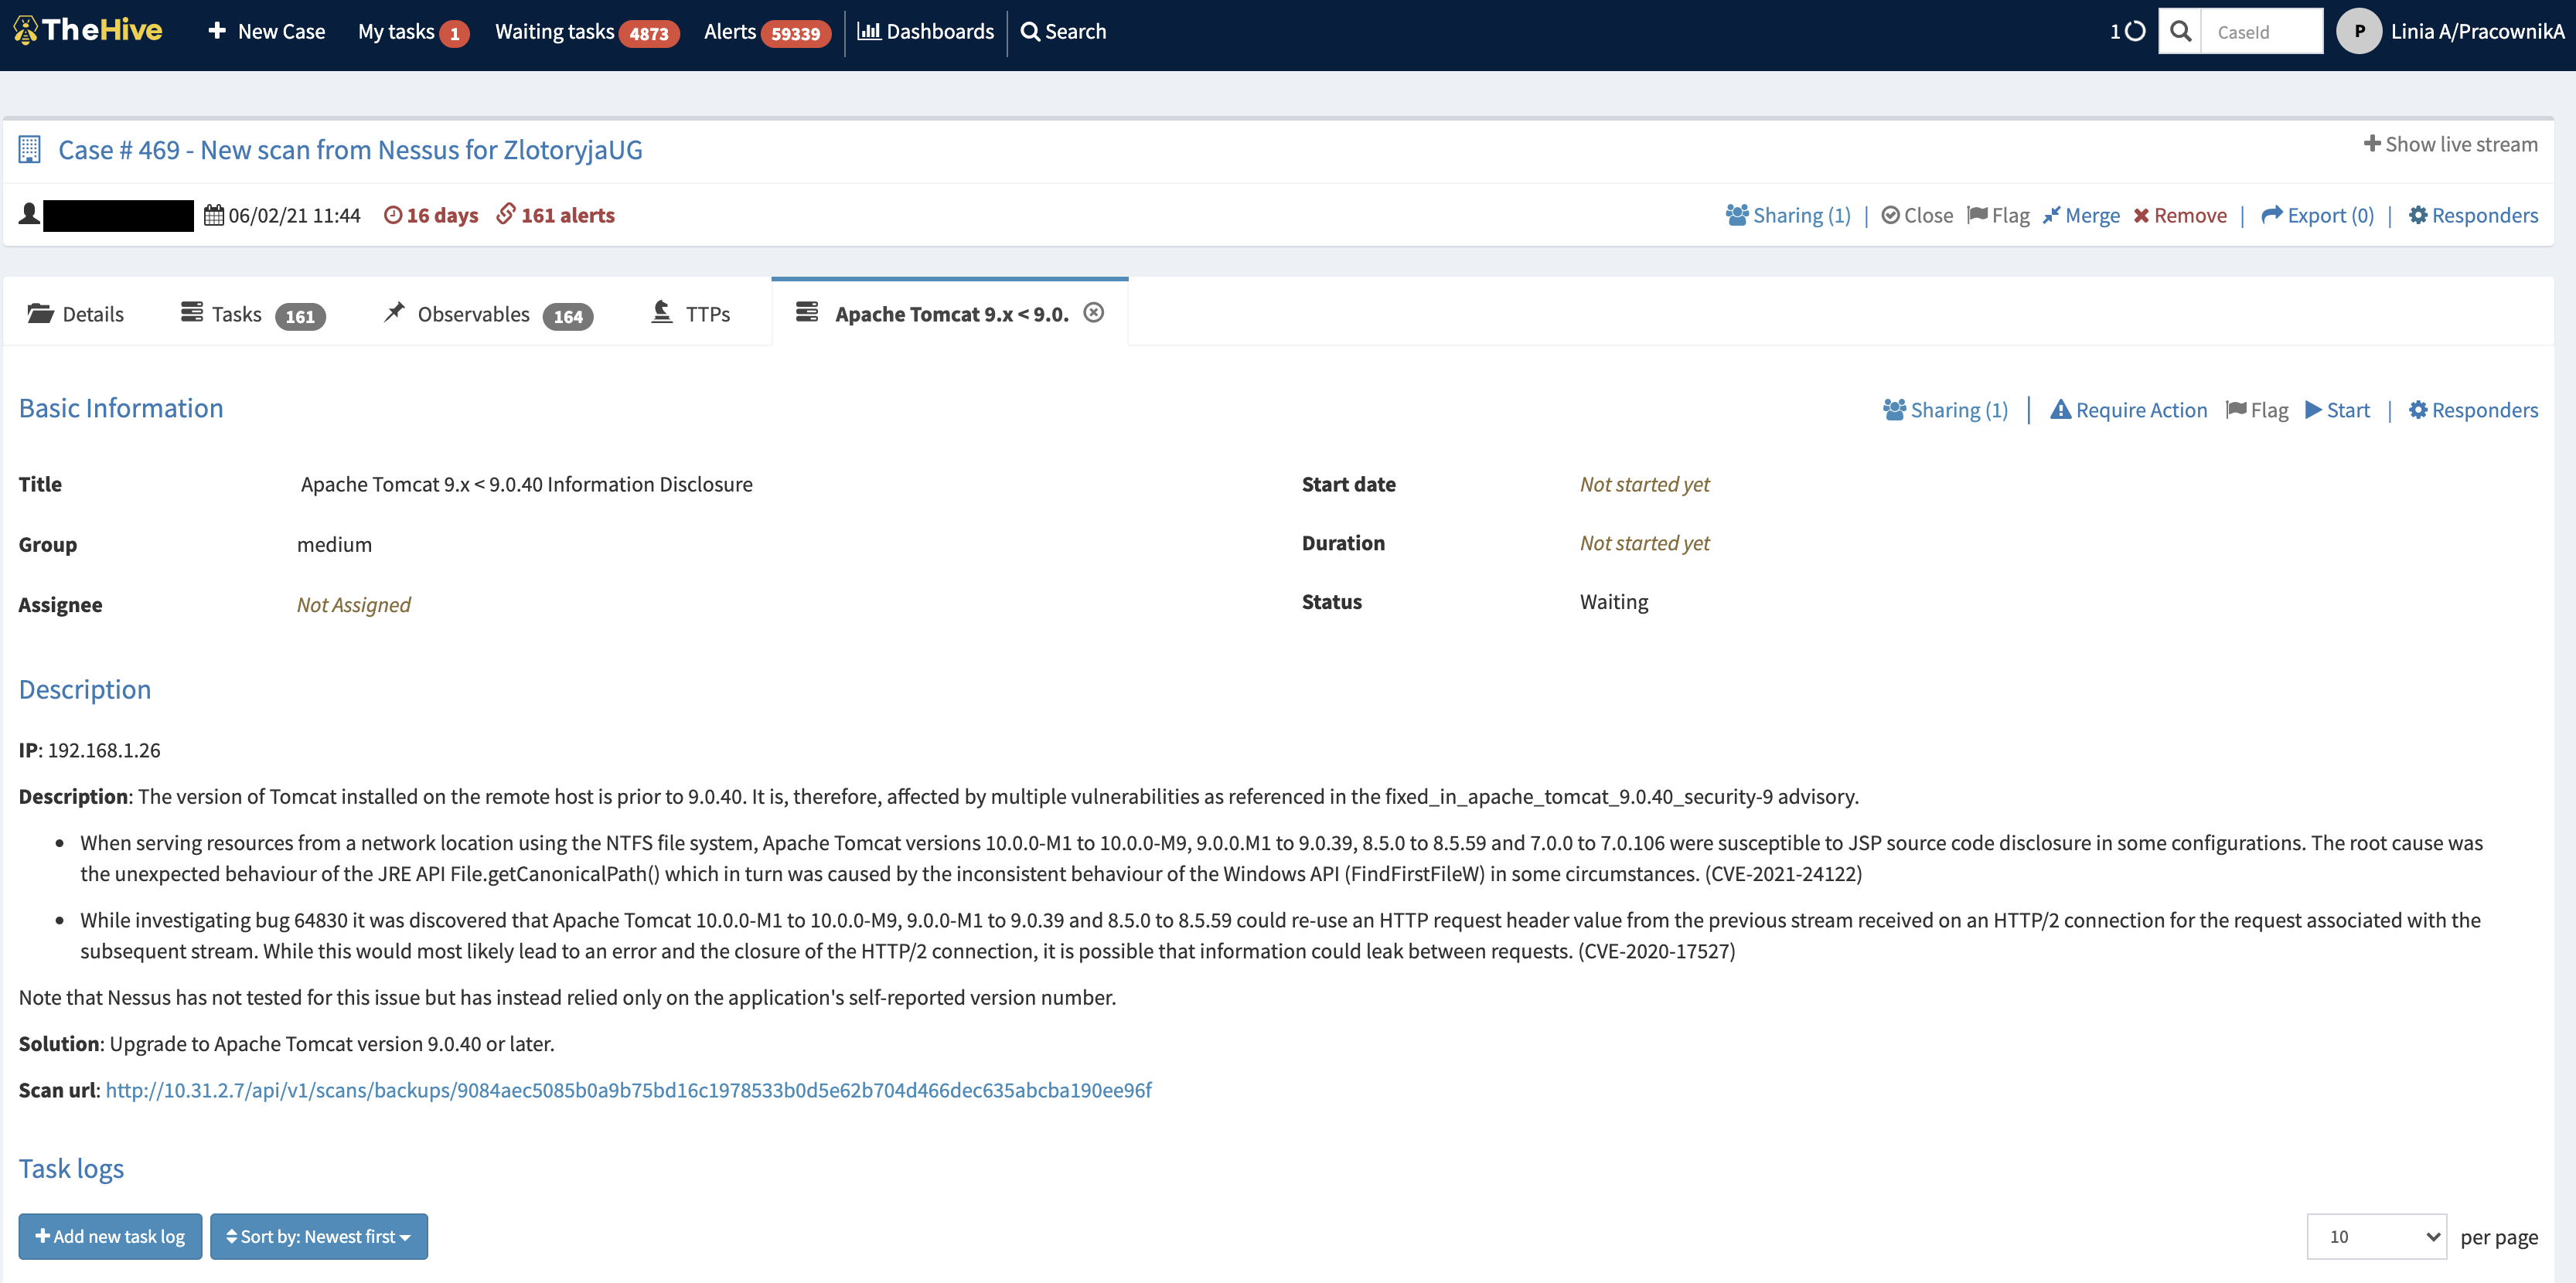
\includegraphics[width=\columnwidth]{Chapters/Rozwiazanie/vmc/hive-sample.png}
\caption{Przykładowy zrzut ekranu oprogramowania Hive zawierający informacje o podatności oraz sposobie jej naprawienia dla administratora zasobu.}
\label{fig:chapter3:hive-sample}
\end{figure}

\bigbreak
Dodatkowo istnieje możliwość wykorzystania modułu Elastalert \cite{elastalert} w celu monitorowania oraz alarmowania o odstępstwach od normy i anomaliach zachodzących w infrastrukturze lub też przygotowanie pełnej automatyzacji pozwalającej na bezpośrednie przesyłanie informacji o podatnościach do odpowiedniego administratora (Rysunek \ref{fig:chapter3:hive-sample}).

%%%%%%%%%%%%%%%%%%%%%%%%%%%%%%%%%%%%%%%%%%%%%%%%

%%%%%%%%%%%%%%%%%%%%%%%%%%%%%%%%%%%%%%%%%%%%%%%%
\subsection{Pobieranie informacji o podatnościach z zewnętrznych źródeł}
W celu rozwiązania problemu opisanego w podrozdziale \ref{sec:modele-zarzadzaia-podatnosciami} dotyczącego aktualizacji informacji dotyczących kategorii bazowej CVSS, która pomimo zapewnień standardu, w rzeczywistości może ulec zmianie, jeśli na jaw wyjdą nowe informacje, zaimplementowano moduł pobierania informacji o podatnościach z publicznych baz danych (ang. Knowledge Collector). Moduł ten odpowiada za pobieranie, aktualizację oraz normalizację informacji z publicznie dostępnych baz danych na temat znanych exploitów, słabości (ang. Common Weakness Enumeration, w skrócie CWE) \cite{martin2007common} oraz podatności (CVE) \cite{cvsspecification}. Do źródeł informacji należą między innymi NVD \cite{booth2013national} i Exploits Database \cite{exploitexploits}. Na rysunku \ref{lst:chapter3:cvedocument} przedstawiono przykładową znormalizowaną strukturę dla podatności, która zawiera również relacje do dokumentów zawierających informacje o publicznie dostępnych exploitach, jak i do informacji o identyfikacji podatnego oprogramowania (ang. Common Platform Enumeration, w skrócie CPE) \cite{buttner2009common}. W dokumencie przechowywany jest cały wektor składający się na ocenę bazową podatności w celu przyspieszenia obliczeń oraz umożliwieniu łatwiejszego wyszukiwania po jej charakterystycznych cechach, np możliwość zdalnego wykorzystania. Po przejściu procesu normalizacji zebrane informacje są możliwe do wyświetlenia w warstwie prezentacji (Rysunek \ref{fig:chapter3:kibana-sample}).

\begin{figure}[thb]
\centering
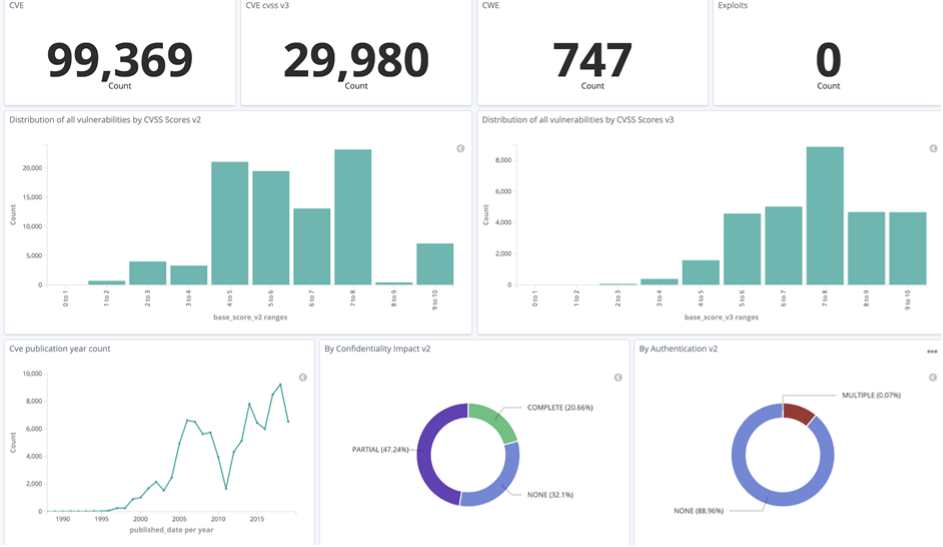
\includegraphics[width=\columnwidth]{Chapters/Rozwiazanie/vmc/kibana-sample.png}
\caption{Przykładowy zrzut ekranu oprogramowania VMC zawierający metryki.}
\label{fig:chapter3:kibana-sample}
\end{figure}

\newpage
\begin{lstlisting}[caption={Przykładowy dokument prezentujący informacje zebrane o podatnościach (ang. CVE) w Elasticsearch.}, label={lst:chapter3:cvedocument}, language=Python, captionpos=b]
class CveDocument:
    id
    base_score_v2
    base_score_v3
    summary
    access_vector_v2
    access_complexity_v2
    authentication_v2
    confidentiality_impact_v2
    integrity_impact_v2
    availability_impact_v2
    attack_vector_v3
    attack_complexity_v3
    privileges_required_v3
    user_interaction_v3
    scope_v3
    confidentiality_impact_v3
\end{lstlisting}

%%%%%%%%%%%%%%%%%%%%%%%%%%%%%%%%%%%%%%%%%%%%%%%%

%%%%%%%%%%%%%%%%%%%%%%%%%%%%%%%%%%%%%%%%%%%%%%%%
\subsection{Pobieranie informacji o zasobach infrastruktury ICT}
\label{sec:cia_desc}
Moduł pobierający informacje o zasobach (ang. Asset Collector) odpowiada za zarządzanie danymi dotyczącymi zasobów wykrytych oraz zdefiniowanych dla monitorowanej sieci \cite{weintraub2016security}. Wykorzystując skonfigurowany przez administratora interwał czasowy, moduł łączy się z bazą zasobów za pomocą interfejsu programistycznego aplikacji (ang. API), udostępnionego przez producentów oprogramowania, następnie stworzony parser wewnątrz VMC przekształca otrzymane informacje do znormalizowanej struktury dokumentu przechowywanego w bazie Elasticsearch.

\bigbreak
Moduł pobierający informacje o zasobach posiada dwa źródła danych. Pierwszym źródłem jest narzędzie Ralph \cite{ralph}, system spełniający wymagania sieci korporacyjnych pozwalających na zarządzanie cyklem życia poszczególnego komponentu środowiska ICT. Drugim źródłem danych jest skaner podatności, który oprócz skanowania posiada funkcjonalność wykrywania komponentów infrastruktury ICT. VMC za pomocą specjalnie przygotowanych reguł (załącznik nr Z.3) pozwala na poinformowanie operatora o niezgodnościach pomiędzy danymi zawartymi w bazie aktywów, a informacjami dostarczonymi z wynikami skanowania. Na rysunku \ref{fig:chapter3:ralph-sample} przedstawiono przykładowe informacje na temat zasobu wykorzystywanego przez organizację. Dodatkowo w bazie aktywów przechowywane są informacje wymagane z punktu widzenie procesu zarządzania podatnościami, takie jak wymagania ciągłości (ang Confidentiality, w skrócie C), integralności (ang. Integrity, w skrócie I) oraz dostępności (ang. Availability, w skrócie A). W kolejnych rozdziałach posłużono się skrótem pochodzącym z języka angielskiego CIA w odniesieniu do wymagań ciągłości, integralności oraz dostępności zasobów, gdyż jest on ogólnie przyjęty w literaturze.


\begin{figure}[thb]
\centering
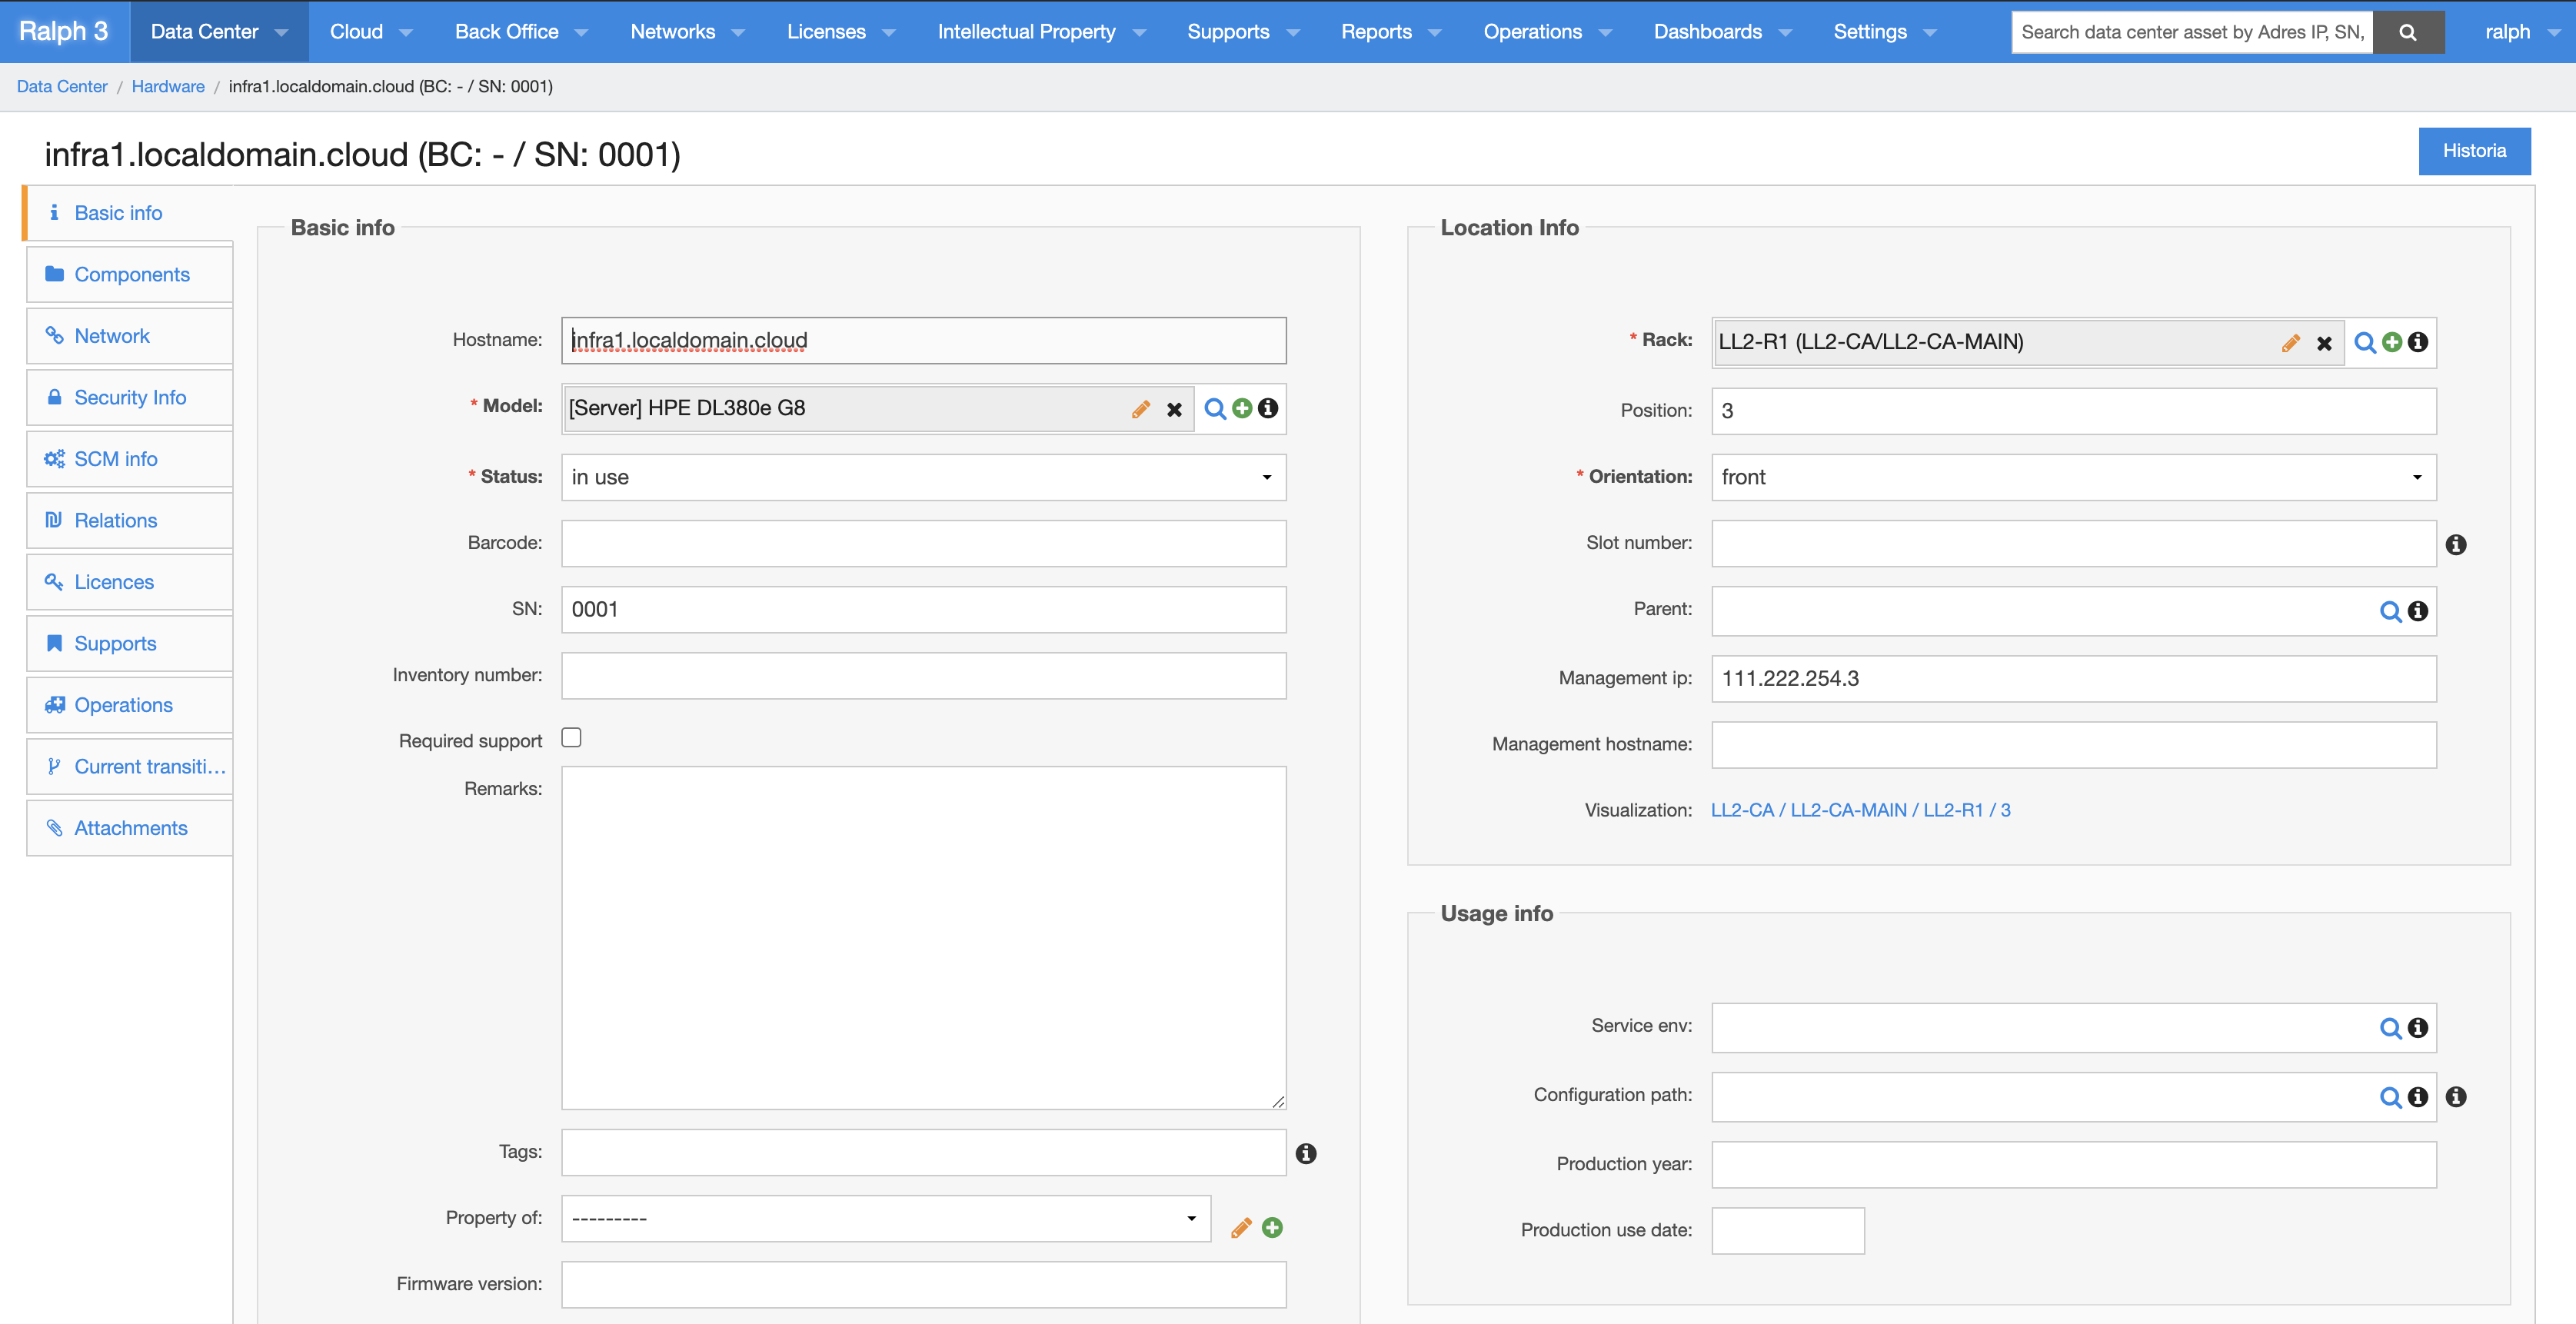
\includegraphics[width=\columnwidth]{Chapters/Rozwiazanie/vmc/ralph-sample.png}
\caption{Przykładowy zrzut ekranu z oprogramowania Ralph.}
\label{fig:chapter3:ralph-sample}
\end{figure}

\bigbreak
Informacje te umożliwiają analitykowi bezpieczeństwa na dostosowanie wyniku oceny podatności w zależności od znaczenia danego zasobu IT dla organizacji, mierzonego pod względem poufności, integralności i dostępności. Oznacza to, że jeśli zasób IT obsługuje funkcję biznesową, dla której dostępność jest najważniejsza, analityk może przypisać większą wartość dostępności w stosunku do poufności i integralności. Każdy wymóg bezpieczeństwa ma trzy możliwe wartości: Niski (ang. Low), Średni (ang. Medium) lub Wysoki (ang. High).

\bigbreak
Pełny wpływ na ocenę środowiskową jest określany przez odpowiednie ustawienia parametrów CIA (należy zauważyć, że ustawienia bazowe CVSS parametrów wpływu na poufność, integralność i dostępność nie ulegają zmianie). Oznacza to, że te parametry modyfikują ocenę środowiskową, zmieniając wagi (podstawowych) metryk wpływu poufności, integralności i dostępności. Na przykład parametr wpływu na poufność ma większą wagę, jeśli wymóg poufności jest wysoki. Podobnie parametr wpływu na poufność ma mniejszą wagę, jeśli wymóg poufności jest niski. Waga parametru wpływu na poufność jest neutralna, jeśli wymóg poufności jest średni. Ta sama logika jest stosowana do wymagań dotyczących integralności i dostępności.

\bigbreak
Listę możliwych wartości przedstawiono w Tabeli \ref{tab:chapter2:cia}. Dla zwięzłości ta sama tabela jest używana dla wszystkich trzech parametrów. Im wyższe wymagania dotyczące bezpieczeństwa, tym wyższa ocena podatności (wartość Średnia jest uważana za domyślną).

\begin{table}[tbh]
\caption{Możliwe wartości parametrów $CIA$}
\begin{center}
\label{tab:chapter2:cia}
\begin{tabular}{lll}
\hline \noalign {\smallskip}
\textbf{Symbol} & \textbf{Wartość} & \textbf{Znaczenie}    \\
\hline \noalign {\smallskip}
L   &   Niskie     & Utrata [poufności/integralności/dostępności] może \\
    &   (ang. Low) & mieć jedynie ograniczony negatywny wpływ na  \\
    &              & organizację lub osoby powiązane z organizacją  \\
    &              & (np. pracowników, klientów).\\
\hline \noalign {\smallskip}
M   & Średnie      & Utrata [poufności/integralności/dostępności] może \\
    & (ang. Medium)& mieć poważny negatywny wpływ na organizację \\
    &              & lub osoby powiązane z organizacją  \\
    &              & (np. pracowników, klientów).\\
\hline \noalign {\smallskip}
H   &  Wysokie     & Utrata [poufności/integralności/dostępności]  \\
    &  (ang. High) & prawdopodobnie będzie miała katastrofalny \\
    &              & negatywny wpływ na organizację lub osoby   \\
    &              & powiązane z organizacją (np. pracowników,  \\
    &              & klientów). \\
\hline \noalign {\smallskip}
ND (CVSS 2.0)& Niezdefiniowane   & Przypisanie tej wartości wskazuje, że nie ma  \\ 
X (CVSS 3.x) & (ang. Not Defined)& wystarczających informacji, aby wybrać \\
                  &                 & jedną z pozostałych wartości, i nie ma wpływu \\ 
                  &                 & na ogólną ocenę środowiskową, tzn. ma taki sam \\
                  &                 & wpływ na ocenę, jak przypisanie wartości średniej. \\
\hline \noalign {\smallskip}
\end{tabular}
\end{center}
\end{table}

%%%%%%%%%%%%%%%%%%%%%%%%%%%%%%%%%%%%%%%%%%%%%%%%

%%%%%%%%%%%%%%%%%%%%%%%%%%%%%%%%%%%%%%%%%%%%%%%%
\subsection{Pobierane informacji o wykrytych podatnościach w infrastrukturze ICT}
Moduł pobierający informacje o wykrytych podatnościach w infrastrukturze teleinformatycznej (ang. Vulnerability Collector) odpowiada za pobieranie, aktualizację oraz normalizację danych ze skanerów podatności Nessus \cite{beale2004nessus} oraz OpenVas \cite{rahalkar2019openvas}. Wykorzystując skonfigurowany przez administratora interwał czasowy, moduł łączy się ze skanerem za pomocą interfejsu programistycznego aplikacji (ang. API) udostępnionego przez producentów oprogramowania skanującego, następnie stworzony parser wewnątrz VMC przekształca otrzymane informacje do znormalizowanej struktury dokumentu przechowywanego w bazie Elasticsearch.

\bigbreak
W celu optymalizacji wyników podczas przetwarzania danych pomijane są podatności sklasyfikowane jako informacyjne. Z raportów dostarczanych ze skanerów podatności pobierane informacje zwierają numer portu, protokół, nazwa usługi, opis podatności oraz informacje, w jaki sposób podatność powinna zostać naprawiona, które stanowią rekomendacje dla osób implementujących mechanizmy naprawcze.


%%%%%%%%%%%%%%%%%%%%%%%%%%%%%%%%%%%%%%%%%%%%%%%%

%%%%%%%%%%%%%%%%%%%%%%%%%%%%%%%%%%%%%%%%%%%%%%%%
\subsection{Metoda optymalizacji obliczeń dla dużej ilości danych}
\label{sec:scaling}
Moduł obliczeniowy (ang. Processing Module) odpowiada za dokonywanie obliczeń oraz aktualizacje oceny wykrytych podatności z uwzględnieniem danych pozyskanych ze wcześniejszych modułów. Obliczenia uruchamiane są za każdym razem, kiedy zostanie wykryta zmiana w przechowywanych danych, pobranych za pomocą modułów opisanych w poprzednich podrozdziałach. Dodatkowo w celu przyspieszenia czasu obliczeń są one wykonywane niezależenie dla każdego klienta (ang. tenant), zachowując pełną separację informacji na temat zagrożeń. Dla każdej nowej lub zaktualizowanej podatności otrzymane wyniki obliczeń zapisywane są w odpowiednich polach dokumentu. Zapisywana jest również informacja, taka jak wektor oceny środowiskowej (ang. Environmental Score Vector), dzięki której można w łatwy sposób przeanalizować każdą z poszczególnych wartości mającą wpływ na końcową ocenę środowiskową.

\bigbreak
Wykorzystując architekturę systemu zaprojektowaną do pracy w chmurze, zaimplementowano algorytm pozwalający na automatyczne wykrywanie ilości dostępnych zasobów w celu ich optymalnego wykorzystania. Po pierwsze, algorytm pobiera liczbę podatności, które nie zostały naprawione lub nie zostały oznaczone jako zmitygowane (Rozdział \ref{sec:proces-zarzadzania-podatnosciami}). Następnie algorytm wyszukuje informacji o systemie, w którym to został uruchomiony, aby ocenić ilość dostępnych zasobów, które można wykorzystać do obliczeń. Podział zadań w zależności od dostępnych zasobów przypisuje się zgodnie z równaniem:

\begin{equation}
d = 
\begin{cases}
\label{eq:chapter3:split_alg}
v//t & \text{jeżeli } v//t \leq t \\
t & \text{w przeciwnym wypadku} 
\end{cases}
\end{equation}
gdzie:
\begin{description}
\item $d$ - ilość danych przetwarzanych przez jeden moduł obliczeniowy
\item $t$ - liczba dostępnych modułów obliczeniowych
\item $v$ - liczba podatności które zostały nienaprawione lub niezmitygowane
\end{description}

\bigbreak
Każdorazowo przed rozpoczęciem procesu obliczeń wykonywane jest powyższe równanie, pozwala to na zastosowanie mechanizmu skalowania horyzontalnego bez potrzeby restartu oprogramowania VMC.

\bigbreak
W celu przyspieszenia obliczeń wartości $TD$ każde zapytanie jest przechowywane w bazie on-memory Redis współdzielonej przez wszystkie moduły obliczeniowe \cite{chen2016towards}, dzięki czemu w rezultacie tylko jeden moduł zliczający wysyła zapytanie do bazy danych, a pozostałe pobierają wcześniej obliczoną informację. Wykonane obliczenia zapisywane są z wykorzystaniem osobnego wątku przy pomocy bulk method \cite{dixit2016elasticsearch}. Dzięki temu pętla obliczeniowa nie jest blokowana na czas zapisu wyników operacji w bazie Elasticsearch. Dodatkowo baza on-memory Redis służy do synchronizacji wszystkich zadań wykonywanych w systemie, pozwalając na tworzenie rozproszonych mutexów oraz semaforów \cite{yadav2015review}. W celu uniknięcia problemów związanych z zakleszczeniem lub zawieszeniem się zadań wykonywanych przez oprogramowanie VMC, zaimplementowano mechanizm kaskadowy, który na wykonanie konkretnego zadania ma trzy próby. Po trzech nie udanych próbach problem z opisem błędu zgłaszany jest do administratora oprogramowania VMC.

%%%%%%%%%%%%%%%%%%%%%%%%%%%%%%%%%%%%%%%%%%%%%%%%

%%%%%%%%%%%%%%%%%%%%%%%%%%%%%%%%%%%%%%%%%%%%%%%%
\subsection{Metoda określania potencjalnych szkód dodatkowych}
\label{sec:cdp}
Parametr określający potencjalne szkody dodatkowe (ang. Colleteral Damage Potential, w skrócie $CDP$) według opisu zamieszczonego w dokumentacji standardu CVSS 2.0 \cite{cvsspecification} odpowiedzialny jest za wskazywanie zasobów infrastruktury IT, które w wyniku chwilowej niedostępności mogą spowodować wysokie straty finansowe dla firmy. Możliwe wartości parametru $CDP$ wraz z opisem wymienione zostały w Tabeli \ref{tab:chapter2:cdp}. 


\bigbreak
Im wyższa wartość parametru, tym większy wpływ na potencjalne zagrożenia, co ma bezpośredni przekład na wyższą ocenę wykrytej podatności. Oczywiście każda organizacja musi sama określić dokładne znaczenie słów „niewielkie, umiarkowane, znaczące i katastrofalne”.

\bigbreak
Na potrzeby obliczeń zaproponowano rozwiązanie napisane w języku Python przedstawione na Rysunku \ref{lst:chapter3:cdp_alg}, gdzie $x$ reprezentuje monitorowany zasób IT, $cr$ jest wymogiem poufności (ang. Confidentiality Requirement), $ir$ oznacza wymóg integralności (ang. Integrity Requirement), $a$ ar oznacza wymóg dostępności (ang. Availability Requirement).

\begin{lstlisting}[caption={Algorytm określający wartość parametru. CDP dla monitorowanego zasobu.}, label={lst:chapter3:cdp_alg}, language=Python, captionpos=b]
 x = [cr, ir, ar]
 if x.count(HIGH) == 3:
        return HIGH
 if x.count(HIGH) > 0:
    return MEDIUM_HIGH

 if x.count(MEDIUM) > 0:
    return LOW_MEDIUM

 if x.count(LOW) > 1:
    return LOW

return NOT_DEFINED
\end{lstlisting}

\begin{table}[tbh]
\caption{Możliwe wartości parametru $CDP$}
\begin{center}
\label{tab:chapter2:cdp}
\begin{tabular}{lll}
\hline \noalign {\smallskip}
\textbf{Symbol} & \textbf{Wartość} & \textbf{Znaczenie}    \\
\hline \noalign {\smallskip}
N  & Żadne              & Brak wpływu na aktywa, produktywność lub przychody \\
   & (ang. None)        & organizacji.\\
\hline \noalign {\smallskip}
L  & Niskie             & Pomyślne wykorzystanie tej podatności może \\
   & (ang. Low)         & spowodować niewielkie  uszkodzenia fizyczne \\
   &                    & lub straty majątkowe. Może wystąpić niewielka \\
   &                    & utrata przychodów lub produktywności organizacji.\\
\hline \noalign {\smallskip}
LM & Niskie-Średnie     & Pomyślne wykorzystanie tej podatności może spowodować\\       
   & (ang. Low-Medium)  & umiarkowane uszkodzenia fizyczne lub straty majątkowe. \\
   &                    &  Może wystąpić umiarkowana utrata przychodów \\
   &                    & lub produktywności organizacji.\\
\hline \noalign {\smallskip}
MH & Średnio-Wysokie    & Pomyślne wykorzystanie tej podatności może spowodować \\
   & (ang. Medium-High) & znaczne szkody fizyczne lub straty materialne. Może \\
   &                    & dojść do znacznej utraty przychodów lub produktywności.\\
\hline \noalign {\smallskip}
H  & Wysokie            & Pomyślne wykorzystanie tej podatności może spowodować \\
   & (ang. High)        & katastrofalne fizyczne lub materialne uszkodzenia. \\ 
   &                    & Może nastąpić katastrofalna utrata  \\
   &                    & przychodów lub produktywności.\\
\hline \noalign {\smallskip}
ND &Niezdefiniowane     & Przypisanie tej wartości do metryki nie wpłynie \\
   & (ang. Not Defined) & na wynik końcowy. \\
\hline \noalign {\smallskip}
\end{tabular}
\end{center}
\end{table}

%%%%%%%%%%%%%%%%%%%%%%%%%%%%%%%%%%%%%%%%%%%%%%%%

%%%%%%%%%%%%%%%%%%%%%%%%%%%%%%%%%%%%%%%%%%%%%%%%
\subsection{Metoda określania dystrybucji podatności}
\label{sec:td}
Parametr określający dystrybucje podatności (ang. Target Distribution, w skrócie $TD$) według opisu zamieszczonego w dokumentacji standardu CVSS 2.0 \cite{cvsspecification} jest specyficzny dla monitorowanego środowiska i odpowiedzialny za wskazanie procentu monitorowanych zasobów IT podatnych na wykryte zagrożenia. Możliwe wartości dla parametru $TD$ są wymienione w Tabeli \ref{tab:chapter2:td}. Im większy odsetek systemów podatnych, tym wyższy wynik końcowy oceny środowiskowej.

\bigbreak
Algorytm obliczający parametr $TD$ został zaimplementowany jako stosunek liczby nienaprawionych i niezmitygowanych podatności do liczby monitorowanych zasobów:

\begin{equation}
TD(x) = 
\begin{cases}
0.00 & x < 0.01 \\
0.25 & 0.01 \leq x < 0.25 \\
0.75 & 0.25 \leq x < 0.75 \\
1.00 & 0.75 \leq x \leq 1.00 \\
\end{cases}
\end{equation}

Gdzie:
\begin{equation}
    x = v / a 
\end{equation}

W powyższym równaniu $v$ reprezentuje liczbę nienaprawionych i niezmitygowanych podatności (Rozdział \ref{sec:proces-zarzadzania-podatnosciami}), natomiast $a$ reprezentuje liczba monitorowanych zasobów w środowisku ICT.

\begin{table}[tbh]
\caption{Możliwe wartości parametru $TD$}
\begin{center}
\label{tab:chapter2:td}
\begin{tabular}{lll}
\hline \noalign {\smallskip}
\textbf{Symbol} & \textbf{Wartość} & \textbf{Znaczenie}    \\
\hline \noalign {\smallskip}
N & Żadne & Nie istnieją żadne systemy docelowe lub cele są tak wysoce      \\
  & (ang. None) & wyspecjalizowane, że istnieją tylko w warunkach \\
  &             & laboratoryjnych. Efektywnie zagrożone jest 0\% środowiska. \\
\hline \noalign {\smallskip}
L & Niskie     & Pomyślne wykorzystanie tej podatności może spowodować \\
  & (ang. Low) & niewielkie uszkodzenia fizyczne lub straty finansowe. \\  
  &            &  Może wystąpić niewielka utrata przychodów  \\
  &            & lub produktywności organizacji. \\
\hline \noalign {\smallskip}
M & Średnie    & Pomyślne wykorzystanie tej podatności może spowodować \\       
& (ang. Medium)& umiarkowane uszkodzenia fizyczne lub straty finansowe.\\
  &           & Może wystąpić umiarkowane utrata przychodów \\
  &           & lub produktywności organizacji.\\
\hline \noalign {\smallskip}
H & Wysokie    & Pomyślne wykorzystanie tej podatności może spowodować \\
  & (ang. High)& katastrofalne fizyczne lub straty finansowe. Może \\ 
  &            & nastąpić katastrofalna utrata przychodów lub produktywności. \\
\hline \noalign {\smallskip}
ND&Niezdefiniowane& Przypisanie tej wartości nie wpłynie na wynik końcowy. \\
  &(ang. Not Defined) & \\
\hline \noalign {\smallskip}
\end{tabular}
\end{center}
\end{table}

%%%%%%%%%%%%%%%%%%%%%%%%%%%%%%%%%%%%%%%%%%%%%%%%

%%%%%%%%%%%%%%%%%%%%%%%%%%%%%%%%%%%%%%%%%%%%%%%%
\section{Metoda konwersji CVSS 2.0 do CVSS 3.x}
\label{sec:ml}
Nie wszystkie publicznie znane podatności mają ocenę bazową według CVSS 3.x, czyli najnowszym i najbardziej zaawansowanej wersji standardu CVSS (Rozdział \ref{sec:modele-zarzadzaia-podatnosciami}). Wynika to z dużej luki czasowej między publikacją standardów CVSS 2.0 i CVSS 3.x, dużej liczbie wykrytych i opublikowanych podatności oraz istotnymi różnicami w sposobie określania właściwości wektorowych oceny bazowej. W związku z tym organizacje korzystające z CVSS do ustalania priorytetów podatności używają obu wersji standardu CVSS i zrezygnowały z pełnego przejścia na CVSS 3.x. W celu rozwiązania niniejszego problemu braku oceny bazowej CVSS 3.x dla wszystkich podatności i umożliwienia wykonania priorytetyzacji wszystkich podatności za pomocą proponowanego modelu środowiskowego CVSS 3.x (Rysunek \ref{fig:chapter1:vm-model-cvss3e}) wykorzystano rozwiązanie zaproponowane przez autora niniejszej rozprawy, natomiast zaimplementowane przez doktora Macieja Nowaka. 

\bigbreak
Konwersja oceny bazowej CVSS 2.0 na CVSS 3.x wymaga jednoczesnego rozwiązania wielu problemów statystycznych. W pozyskiwanych danych wejściowych występuje niezrównoważenie (ang. imbalance data) powodujące trudności w fazie uczenia, co skutkuje obniżeniem zdolności predykcyjnych. Dodatkowo wynik końcowy CVSS 3.x powiązany jest funkcją opisaną 8 parametrami, z których każdy może przyjmować jedną z kilku wartości (od 2 do 4), ale pozyskanie samych parametrów tworzących wektor CVSS 2.0 dla większości przypadków okazuje się niewystarczające.

\bigbreak
Liczba kombinacji występująca w wektorze używanym do wyliczenia oceny bazowej CVSS 3.x wynosi 2592, natomiast wartość tego wektora zawiera się w przedziale 0 – 10 z rozdzielczością wynoszącą 0.1. Inaczej mówiąc, na podstawie zbioru uczącego, finalnie trzeba dokonać klasyfikacji każdego wektora testującego do jednej ze stu klas przypisanych do oceny bazowej CVSS 3.x.

\bigbreak
Zgodnie z dokumentacją opisującą ocenę bazową CVSS 3.x wyliczona wartość oceny bazowej przyjmuje jedną z pięciu kategorii (ang. Qualitative Severity Rating Scale). Kategorie te również nie są tak samo liczne, a ich proporcja wynosi odpowiednio: 1 : 39 : 30 : 20 : 10 (informacyjna : niska : średnia : wysoka : krytyczna).  W praktyce wskazana asymetria zakresu kategorii oznacza, że jeśli ocena bazowa CVSS dla wersji 3.x przyjmuje wartość 0, to wykonując konwersję z oceny bazowej CVSS 2.0 na 3.x, nie możemy popełnić żadnego błędu. Odchylenie od oceny bazowej CVSS 3.x dla kategorii krytycznej musi być z kolei mniejsze niż dla wysokiej, itd. 

\bigbreak
Podejście do rozwiązania problemu konwersji oceny bazowej składa się z kilku kroków. Po pierwsze, z pozyskanych danych należy odpowiednio wyselekcjonować zbiory trenujące tak, aby uzyskać jak najwyższą sprawność (ang. accuracy) klasyfikacji dla każdego z ośmiu parametrów tworzących wektor CVSS 3.x. W tym celu zastosowano dwie koncepcje wykorzystujące medianę i korelację wektorów, z których pierwsza, poprzez zastosowanie undersamplingu prowadzi do pełnego zbalansowania danych, natomiast druga statystycznie wiąże wszystkie parametry wektora CVSS 3.x, pozwalając na pozyskanie wektorów uczących z pewną stałą regułą. Kolejnym krokiem jest wyodrębnienie cech (ang. relevant features) z zestawu pozyskanych wektorów, używając analizy głównych komponentów (ang. Principal Component Analysis, w skrócie PCA), a następnie wykonanie uczenia pod nadzorem (ang. supervised learning methods) za pomocą różnych algorytmów. Porównano i przeanalizowano wiele metod statystycznej klasyfikacji (ag. statistical classification methods), takich jak maszyna wektorów podpierających (ang. Support Vector Machine, w skrocie SVM), naiwny klasyfikator Bayesa (ang. Naive Bayes classifier) oraz k-najbliższych sąsiadów (ang. K-nearest neighbor, w skrócie kNN). Po ustaleniu, które metody najskuteczniej klasyfikują w obrębie danego parametru wektora CVSS 3.x, przeprowadzano próby klasyfikacji przy zwiększeniu liczby wektorów zbioru testującego ze 100 do 1000. To ostatecznie pozwoliło wybrać najlepszych kandydatów i odpowiednio zoptymalizować modele klasyfikacji.

\bigbreak
Wstępne badania wykazały, że oryginalne wektory oceny bazowej CVSS 2.0 zostały nieprawidłowo zmapowane do 3.x, więc oryginalny wektor oceny bazowej CVSS 2.0 został rozszerzony o dodatkowe 50, 100, 500 i 1000 elementów. Dodatkowe elementy są uzyskiwane z opisów podatności i obliczane poprzez podzielenie liczby wystąpień słów kluczowych przez 100. Przetwarzanie tekstu zostało wykonane przy użyciu biblioteki Natural Language Toolkit (NLTK) \cite{bird2009natural}. Skrypty i dane wejściowe zostały umieszczone w repozytorium otwartego dostępu \cite{cvss-2-extended-vector-database-github}. Ponieważ uzyskane dane są niezrównoważone, zastosowano metodę undersamplingu opisaną w \cite{Nowak-cldd-2021}. Badania zostały przeprowadzone z następującymi algorytmami uczenia maszynowego:
\begin{itemize}
\item Algorytm k-najbliższych sąsiadów (ang. k-Nearest Neighbors, w skrócie kNN) z metryką euklidesową (E) i podobieństwem cosinusowym (C).
\item Naiwny klasyfikator Bayesa (ang. Naive Bayes classifier, w skrócie NB).
\item Probabilistyczna sieć neuronowa (ang. Probabilistic Neural Network, w skrócie PNN),
\item Miękkie niezależne modelowanie według analogii klas (ang. Soft Independent Modeling of Class Analogy, w skrócie SIMCA),
\item Maszyna wektorów podpierających z funkcją jądrową (ang. Kernel support vector machine, w skrócie KSVM) w dwóch konfiguracjach — z liniową funkcją jądra i korzystającą z jądra uczącego z radialną funkcją bazową (TGRBF) \cite{nowak2019recognition}. KSVM TRGBF w pętli uczenia wykorzystuje 2-krotną walidację krzyżową (2-krotne CV), współczynnik błędnej klasyfikacji (ang. Misclassification Ratio, w skrócie MCR), algorytm NM z zestawem 50 punktów początkowych i kNN z metryką cosinusową (C) do końcowej klasyfikacji nierozpoznanych próbek. Dodatkowo w przypadku KSVM TRGBF zastosowano podejście One-vs-One (OvO) dla parametrów o co najmniej 3 klasach.
\end{itemize}

Optymalizacja parametrów algorytmów uczenia maszynowego została przeprowadzona na podstawie pięciokrotnej walidacji krzyżowej zbioru 100 elementowego. Procedura testowa została powtórzona 10 razy i pozwoliła na określenie uśrednionych wartości współczynnika błędnych klasyfikacji (ang. Misclassification Ratio, w skrócie MCR), precyzji (ang. precision), czułości (ang. recall) i F1 (średnia harmoniczna pomiędzy precyzją (ang. precision) i czułością (ang. recall)). W kolejnym etapie wykonana została ocena dokładności klasyfikacji dla wybranych algorytmów na podstawie 30 prób przeprowadzonych z zbiorami testowymi zawierającymi losowo wybranymi 1000 elementowymi wektorami. Parametry algorytmu zostały ponownie zoptymalizowane w celu uzyskania maksymalizacji dokładności klasyfikacji przy jak najmniejszym rozrzucie wyników. Opisane w rozdziale 4 wyniki zostały potwierdzone za pomocą zbioru testującego składającego się z zbioru 71 000 wektorów.

%%%%%%%%%%%%%%%%%%%%%%%%%%%%%%%%%%%%%%%%%%%%%%%%

%%%%%%%%%%%%%%%%%%%%%%%%%%%%%%%%%%%%%%%%%%%%%%%%
\begin{comment}
\section{Metoda pomiaru zakresu oraz liczby zmian w ocenie podatności}
\label{sec:metoda_pomiar_zakres_oraz_liczba_zmian}
W celu zmierzenia zakresu oraz liczby zmian w ocenie podatności a tym samym wpływu parametrów środowiskowych $CIA$, $TD$ oraz $CDP$ na ocenę bazową CVSS, posłużono się równaniem przedstawionym poniżej:

\begin{equation}
d = X_{CVSS_{Base}} - X_{CVSS_{Env}}
\end{equation}

Gdzie wartość $d$ to różnica pomiędzy otrzymanymi ocenami, $X_{CVSS_{Base}}$  to ocena bazowa otrzymana ze skanera Nessus, $X_{CVSS_{Env}}$ to ocena środowiskowa obliczona za pomocą oprogramowania VMC. Otrzymana ujemna wartość $d$ wskazuje, że ocena środowiskowa została obniżona w stosunku do oceny bazowej, analogicznie, wartość dodatnia $d$ informuje, że ocena środowiskowa jest wyższa od ceny bazowej. W celu określenia liczby zmian w priorytetyzacji podatności dla standardu CVSS 2.0 oraz CVSS 3.x, zliczono wszystkie unikalne wystąpienia otrzymanych wartości $d$.
\end{comment}
